\documentclass[conference]{IEEEtran}

\usepackage{amsmath, amsthm, amssymb, dsfont, accents}

\usepackage{tikz,pgfplots}
\usepackage{hyperref, booktabs}
\usepackage{biblatex}

\pgfplotsset{compat=1.14}

\usetikzlibrary{calc, automata}
\newlength\figureheight
\newlength\figurewidth

\addbibresource{2_references.bib}

\pdfinfo{
   /Author (Homer Simpson)
   /Title  (Robots: Our new overlords)
   /CreationDate (D:20101201120000)
   /Subject (Robots)
   /Keywords (Robots;Overlords)
}

% MDPs
\newcommand{\MDP}{\mathbb{M}}

\newcommand{\X}{\mathbb{X}}
\newcommand{\U}{\mathbb{U}}
\newcommand{\init}{\rho}
\newcommand{\tr}{T}

\newcommand{\pol}{\mu}

% LTL
\newcommand{\True}{\texttt{true}}
\newcommand{\False}{\texttt{false}}
\newcommand{\AP}{AP}

\newcommand{\ltluntil}{\mathcal{U}}
\newcommand{\ltlnext}{\bigcirc}

\newcommand{\alphabet}{{2^{\AP}}}
\newcommand{\word}{\boldsymbol{\pi}}
\newcommand{\letter}{\pi}
\newcommand{\lab}{L}

\newcommand{\FSA}{\mathcal{A}}

% Probability
\newcommand{\Prob}{\mathbf{P}}


% Value iteration
\newcommand{\bellman}{\mathcal{B}}


% Math
\DeclareMathOperator*{\argmin}{arg\,min}
\DeclareMathOperator*{\argmax}{arg\,max}
\newcommand{\ind}{\mathbf{1}}


\newtheorem{problem}{Problem}
\newtheorem{definition}{Definition}
\newtheorem{remark}{Remark}
\newtheorem{example}{Example}

\newcommand{\red}[1]{{\color{red} #1 }}
\newcommand{\sofie}[1]{{\color{orange}[ #1 ]}}
\begin{document}

%\title{\huge Sequential Value Iteration for Modular Systems Applied to Collaborative Space Robotics}

%\title{\huge Specification-oriented Active Exploration via Sequential Dynamic Programming: Applications to Space Exploration via a Rover-Copter Team}

%\title{\huge Specification-guided Active Exploration: Applications to Safety-critical Mars Rover-Copter Mission}

\title{\huge Specification-guided Active Exploration: Applications to a Risk-averse Rover/Copter Mars Mission}

%\title{\huge Verifiability-oriented Active Exploration: Applications to Safety-critical Mars Rover-Copter Team}

%\title{\huge Satisfaction-oriented Active Exploration: Applications to Safety-critical Mars Rover-Copter Team}

\author{PN et al}

\maketitle

\begin{abstract}
  As a step towards achieving autonomy in space exploration missions, we consider a collaborative robotic system with a copter and a rover. The copter explores an unknown environment so as to maximize the probability that the rover can satisfy a science mission expressed in Linear Temporal Logic. We mitigate the curse of dimensionality for this large system by leveraging its decomposed nature, and by using sparse tensor product representations for value function and control policy. With hardware experiments, we demonstrate that the resulting policy makes intelligent decisions in the face of uncertainty.
\end{abstract}

\IEEEpeerreviewmaketitle

	
%%%%%%%%%%%%%%%%%%%%%%%%%%%%%%%%%%%%%%%%%%%%%%%%
%%%%%%%%%%%%%%%%%%%%%%%%%%%%%%%%%%%%%%%%%%%%%%%%

\section{Introduction}

\begin{itemize}
  \item Main (potential) contributions:
  \begin{itemize}
    \item Reactive control in environment belief space
    \item Contract with low-level safety-critical? controller
    \item Cooperative robotics (copter explores to maximize probability that rover can satisfy spec)
    \item Efficient sequential value iteration for product MDPs
    \item More difficult: label-based abstraction for quadrotor (belief or non-belief) dynamics?? 
  \end{itemize}
  \item Other ideas
  \begin{itemize}
  	\item Abstract systems to MDPs modularly based on relative degree (e.g. velocities and positions) and connect the resulting MDPs in series. Problem: connection not sparse. What is continuous analogue?
  \end{itemize}
\end{itemize}

\begin{itemize}
  \item Work for literature review
  \begin{itemize}
    \item \cite{Papusha2016}
    \item \cite{Alora2016}
    \item Maybe (need to read): \cite{Lavaei2017}
    \item read this earlier work too: \url{https://arxiv.org/abs/1507.00509} Also there is a reference in this paper to work they build on that has been developed for belief space models.
  \end{itemize}
\end{itemize}

\subsection{Preliminaries}

\begin{itemize}
  \item $\mathcal P(\X)$: probability densities \sofie{[or distributions?]} over $\X$
\end{itemize}

\subsection{Paper layout}

\section{Markov Decision Processes and Temporal Logics}

We give definitions related to Markov Decision Process (MDPs), followed by basic concepts related to linear temporal logics.

\subsection{Markov Decision Processes}

We first define Markov decision processes over finite state spaces as follows \cite{hll1996}.
% \cite{mt1993,bertsekas2004stochastic}.
\begin{definition}
\label{def:MDP}
  A discrete-time \textbf{Markov decision process} (MDP) is a tuple $\MDP = (\X, \init, \tr, \U)$ where
  \begin{itemize}
    \item $\X$ is a (finite) state space with states $x\in\X$; % as its elements;
    \item $\init \in \mathcal P(\X)$ is an initial probability distribution; \sofie{Needed? we could give a fixed initial condition.}
    \item $\U$ is a (finite) input space with inputs $u\in\U$;
    \item $\tr$ is a conditional stochastic kernel that assigns to each state $x\in \X$ and control $u\in \U$ a probability density $\tr(\cdot\mid x,u)$ over $\X$.
  \end{itemize}
\end{definition}
\sofie{I'd refer to probability distributions.  The notion $x_{k+1} \sim \tr(\cdot \mid x_k, u_k)$ doesnt hold for a density. As alternative the probability distribution $T(\cdot)$ with the associated probability density distribution$t$ such that $ T(A)=\int_A t(x)dx$.}
An execution of $\MDP$ is a state-input sequence $(x_0, u_0)(x_1, u_1)\ldots$ where $x_0 \sim \rho$ and $x_{k+1} \sim \tr(\cdot \mid x_k, u_k)$ for inputs $u_k \in \U$. 

\subsection{Specifications}

\begin{itemize}
  \item Something about atomic propositions (and examples)
\end{itemize}

Consider a set $AP = \{ p_1, \ldots, p_L \}$ of atomic propositions; it defines an \emph{alphabet} $\alphabet$ where each \emph{letter} $\letter$ of the alphabet is defined as a set of atomic propositions. An infinite string of letters is a \emph{word} $\word=\letter_0\letter_1\letter_2\ldots\in\alphabet^{\mathbb{N}}$.

To quantify the dynamic behavior of a system, we define the word associated to an MDP execution. Consider a labeling function $\lab: \X \rightarrow \alphabet$ that maps states to letters in the alphabet. The words generated by a belief \sofie{[define belief states beforehand?]}trajectory $\mathbf{x} = x_0 x_1 x_2 \ldots$ can be defined as the word $\word = \lab(x_0)\lab(x_1) \lab(x_2) \ldots$. System properties can now be expressed via temporal logic formulas over the generated words.

Properties are formulas composed of atomic propositions and operators. In the sequel we focus on a fragment of linear temporal logic. 
\begin{definition}
  \label{def:gdtl-syntax}
  Formulas in the \textbf{syntactically co-safe LTL} (scLTL) fragment are constructed according to the grammar
  \begin{equation*}
    \label{eq:scLTL}
    \psi =  \True \ |\ p \ |\ \lnot p \ |\ \psi_1 \vee\psi_2  \ |\ \psi_1 \land \psi_2 \ |\ \psi_1 \ltluntil \psi_2 \ |\ \ltlnext \psi,
  \end{equation*}
  where $p\in \AP$ is an atomic proposition.
\end{definition}

% The syntax defines the symbols and their correct ordering to form a formulae.
To define the interpretation of a formula, i.e. the \emph{semantics}, consider a word $\word$.

\begin{definition}
 The \textbf{semantics} of scLTL are defined recursively as follows: $\word$ \textbf{satisfies} $\psi$ at time $k$, written $(\word, k) \models \psi$, if
 \begin{itemize}
    \item $(\word, k) \models \True$;
    \item $(\word, k) \models p$ iff $p \in \letter_k$;
    \item $(\word, k) \models \psi_1 \land  \psi_2  $ iff $ ( (\word, k) \models \psi_1 ) \land ( (\word, k) \models \psi_2 ) $;
    \item $(\word, k) \models \psi_1 \lor  \psi_2  $ iff $ ( (\word, k) \models \psi_1 ) \lor ( (\word, k) \models \psi_2 ) $;
    \item $(\word, k) \models  \psi_1 \ltluntil \psi_2 $ iff $\exists j \geq k \text{ s.t. } ((\word, j) \models \psi_2 ) $ and $(\word, l) \models \psi_1, \forall l \in \{k, \ldots j-1\}$;
    \item $(\word, k) \models \ltlnext \psi$ iff $(\word, k+1) \models \psi$.
 \end{itemize}

\end{definition}

We say that a trajectory $\mathbf{x} = x_0 x_1 x_2 \ldots$ satisfies a specification $\psi$, written $\mathbf{x} \models \psi$, if the generated word $\word =\lab(x_0) \lab(x_1) \lab(x_2) \ldots$ satisfies $\psi$ at time 0, i.e. $\word_0 \models \psi$.

\subsection{Problem Statement}

The objective of this work is to design a policy $\pol$ such that a specification $\psi$ is satisfied with a given probability.
\begin{problem}
\label{prob:main}
  Consider a model $\MDP = (\X, \rho, \tr, \U)$ generating trajectories $\mathbf{b} = x_0 x_1 x_2 \ldots$, a labeling function $\lab : \X \rightarrow AP$, and a scLTL formula $\psi$ defined over $AP$. Construct a policy $\pol$ such that
  \begin{equation}\label{eq:probstatement}
    \Prob_\init^\pol ( \mathbf{b} \models \psi )\geq p,
  \end{equation}
  where $p$ is either given or to be maximized.
\end{problem}

\subsection{Policy Synthesis via Value Iteration}

Policy synthesis for a scLTL specification over a space $\X$ is equivalent to reachability of $\X\times Q_f$ on the product system $\MDP \otimes \FSA_\psi$. In this case, the Bellman operator is
\begin{equation}
\label{eq:V_recopt_inf_mu}
%\begin{aligned}
  \bellman_\pol (\mathbf V)(b,q)\! = \hspace{-1mm} \int_{\X} \hspace{-1mm} \max \left( \mathbf 1_{Q_f}(q'), \!\mathbf V( b'\!, q') \right)\! {\tr}(\mathrm{d} b' |b,\pol(b,q))\!
%\end{aligned}
\end{equation}
with the implicit DFSA transitions  $q' =\delta_\FSA(q,\lab(b'))$, %\red{$\mathrm{d} b'= d b'\times\{q'\}$},
and similarly for the policy-optimal version $\bellman_*$.  For the converged value function $\mathbf V^\infty_* =  \lim_{K\rightarrow\infty}\bellman_*^K\! \mathbf V^0$, now expresses the value of
\begin{equation}
\label{eq:prob:_optimal} 
 \sup_{\pol}\mathbf{P}_\init^{\pol}( {\mathbf{b}} \vDash\! \psi)\! =\!
  \int_{\X} \! \max \left( \mathbf 1_{Q_f}( q'), 
   \mathbf V^\infty_*(x_0, q') \right) \init(\mathrm{d} x_0) \!
\end{equation}
with the associated deterministic and stationary policy $ \pol_*=(\pol_*,\pol_*,\ldots)$ obtained as the maximizing argument. 
This policy defined for the product MDP $\MDP \otimes \FSA_\psi$, maps to control actions as a function of the state $(b,q) \in \X \times Q$, and can be translated to a non-stationary policy for the original MDP $\MDP$ that includes $\FSA_\psi$ as a memory model.


\section{Sequential Value Iteration}
\label{sec:sequential_val_iter}


\subsection{Networks of MDPs}

Consider two MDPs $\MDP_1 = (\X_1, \init_1, \U_1, \tr_1)$ and $\MDP_2 = (\X_2, \init_2, \U_2, \tr_2)$. Next we introduce the parallel and serial products between the two.
\begin{definition}
  The \textbf{parallel product} of $\MDP_1$ and $\MDP_2$ is the MDP 
  \begin{equation}
    \MDP_1 \otimes_{par} \MDP_2 = (\X_1 \times \X_2, \init_{par}, \U_1 \times \U_2, \tr_{par}),
  \end{equation}
  where
  \begin{equation}
    \init_{par}(x_1, x_2) = \init_1(x_1) \init_2(x_2)
  \end{equation}
  and
  \begin{equation}
  \begin{aligned}
      \tr_{par}&(x_1', x_2' \mid x_1, x_2, u_1, u_2) \\
      & = \tr_1 (x_1' \mid x_1, u_1) \tr_2 (x_2' \mid x_2, u_2)
  \end{aligned}
  \end{equation}
\end{definition}

\begin{definition}
  The \textbf{serial product} of $\MDP_1$ and $\MDP_2$ given a \textbf{connection} $C : \X_1 \rightarrow \U_2$ is the MDP 
  \begin{equation}
    \MDP_1 \otimes_{ser} \MDP_2 = (\X_1 \times \X_2, \init_{ser}, \U_1, \tr_{ser}),
  \end{equation}
  where
  \begin{equation}
    \init_{ser}(x_1, x_2) = \init_1(x_1) \init_2(x_2)
  \end{equation}
  and
  \begin{equation}\label{eq:serial}
  \begin{aligned}
      \tr_{ser}&(x_1', x_2' \mid x_1, x_2, u_1) \\
      & = \tr_1 (x_1' \mid x_1, u_1) \tr_2 (x_2' \mid x_2, C(x_1') )
  \end{aligned}
  \end{equation}
\end{definition}
That is, a transition $x_1 \rightarrow x_1'$ in $\MDP_1$ triggers an action $C(x_1')$ in $\MDP_2$ that results in a transition in $x_2' \sim T_2(\cdot \mid x_2, C(x_1'))$

\begin{itemize}
  \item \red{Can we do more general MDP graph?}\sofie{What do you mean with this question?}
\end{itemize}

\subsection{Sequential Iteration of Bellman Operator}

\begin{itemize}
  \item \red{Can we include action in Bellman op?}\sofie{Do you mean to do a Q-iteration? Have a value function that ranges over both action and state? This could be troublesome as it would increase the size of the value function.}
\end{itemize}

Given a function $g: \X \times \mathbb{R}_+ \rightarrow \mathbb{R}_+$, consider a general Bellman operator $\bellman : (\X \rightarrow \mathbb{R}_+) \rightarrow (\X \rightarrow \mathbb{R}_+)$ on the following form:
\begin{equation}
  (\bellman V) (x) = \max_{\pol \in (\X \rightarrow \U)} \sum_{x' \in \X}  g(x', V(x')) T(x' \mid x, \pol(x)).
\end{equation}
\sofie{Define the set of allowed policies : $\mathbf \Pi$ the set of measurable functions mapping from $\X$ to $\U$.  You cannot take any possible function due to measurability issues.  }
The optimal value function $V^*$ and policy $\pol^*$ for a given bellman operator $\bellman$ is found via the iterations
\begin{subequations}
\label{eq:value_iter}
  \begin{align}
    & V^*_0 \equiv 0, \\
    & V^*_{k+1}  = \bellman V_k \label{eq:iter}, \\
    & \pol^* \in \argmax_{\pol \in (\X \rightarrow \U)} \sum_{x' \in \X}  g(x', V^*(x')) T(x' \mid x, \pol(x)).
  \end{align}
\end{subequations}

\begin{example}
  For the Bellman operator corresponding to reaching a set $X_f$, the function $g$ is given by
  \begin{equation*}
    g(x', v') = \max( \ind_{X_f}(x'), v').
  \end{equation*}
\end{example}

\begin{example}
  Consider the finite-horizon optimal control problem 
  \begin{equation}
     \max \sum_{t=0}^T J_t(x_t).
  \end{equation} 
  In this case, if the dynamic programming is initialized with $V_T(x) = J_T(x)$, iterated applications of the Bellman operator corresponding to $g_t(x', v') = J_{t-1}(x') + v'$, i.e.
  \begin{equation*}
    V_{t-1}(x) = \bellman_t V_{t} (x) = \max_{\pol} (J_{t-1}(x') + V_{t}(x')) T(x' \mid x, \pol(x))
  \end{equation*}
  computes the value function at times $T-1, T-2, \ldots, 0$.
\end{example}

We now consider the Bellman iteration step for parallel and serial product MDPs. For a parallel MDP we get
\begin{equation*}
\begin{aligned}
  \max_{\pol: (\X_1 \times \X_2 \rightarrow \U_1 \times \U_2)} \sum_{x_1', x_2' \in \X_1 \times \X_2}  g(x_1', x_2', V^*(x_1', x_2')) \\
  \times T_{par}(x_1', x_2' \mid x_1, x_2, \pol(x_1, x_2)) \\
  = \max_{\pol: (\X_1 \times \X_2 \rightarrow \U_1 \times \U_2)} \sum_{x_1' \in \X_1} T_1(x_1' \mid x_1, \pol(x_1, x_2)) \\
    \sum_{x_2' \in \X_2}  g(x_1', x_2', V(x_1', x_2')) T_2(x_2' \mid x_2, \pol(x_1, x_2)).
\end{aligned}
\end{equation*}
It follows that the Bellman update $V \mapsto \bellman V$ for a parallel product can be computed sequentially as follows:
\begin{equation}
\begin{aligned}
  W_2(x_1', x_2') &= g(x_1', x_2', V(x_1', x_2')) \\
  W_1(x_1, x_1', x_2) &=\\ &\hspace{-1cm} \max_{\pol_2: \X_1 \times \X_2 \rightarrow \U_2} \sum_{x_2' \in \X_2}  T_2(x_2' \mid x_2, \pol_2(x_1, x_2)) W_2(x_1', x_2')  \\
  \bellman V(x_1, x_2) &=\\ &\hspace{-1cm}  \max_{\pol_1: \X_1 \times \X_2 \rightarrow \U_1}  \sum_{x_1' \in \X_1}  T_1(x_1' \mid x_1, \pol_1(x_1, x_2)) W_1(x_1', x_2)
\end{aligned}
\end{equation}
\red{
\begin{itemize}
  \item Decomposition requires that $W_1$ is independent of $x_1$. Satisfied if:
  \begin{itemize}
    \item Decentralized policy is optimal. When is this true?
    \item We consider policy $\mu_2 = \mu_2(x_1', x_2)$ (i.e. $\MDP_1$ moves first).
    \item If there is no policy maximization (e.g., if it is part of a serial product)
  \end{itemize}
\end{itemize}

}

For a serial product we get
\begin{equation*}
\begin{aligned}
  \bellman V (x_1, x_2) & = \max_{\pol: (\X_1 \times \X_2 \rightarrow \U_1)} \sum_{x_1', x_2' \in \X_1 \times \X_2}  g(x_1', x_2', V(x_1', x_2')) \\
  & \quad \times T_{ser}(x_1', x_2' \mid x_1, x_2, \pol(x_1, x_2)) \\
  & = \max_{\pol: (\X_1 \times \X_2 \rightarrow \U_1)} \sum_{x_1' \in \X_1} T_1(x_1' \mid x_1, \pol(x_1, x_2)) \\
  & \quad \times \sum_{x_2' \in \X_2}  g(x_1', x_2', V(x_1', x_2')) T_2(x_2' \mid x_2, C(x_1')).
\end{aligned}
\end{equation*}
It follows that the Bellman update $V \mapsto \bellman V$ for a serial product can be computed sequentially as follows:
\begin{equation*}
\begin{aligned}
  W_2(x_1', x_2') & = g(x_1', x_2', V(x_1', x_2')) \\
  W_1(x_1', x_2) & = \sum_{x_2' \in \X_2}  T_2(x_2' \mid x_2, C(x_1')) W_2(x_1', x_2'), \\
  \bellman V(x_1, x_2) & = \max_{\pol: (\X_1 \times \X_2 \rightarrow \U_1)} \sum_{x_1' \in \X_1} T_1(x_1' \mid x_1, \pol(x_1, x_2)) W_1(x_1', x_2).
\end{aligned}
\end{equation*}
As a consequence, the Bellman recursion can be computed without computing the transition matrices for the aggregate system $\MDP_1 \otimes_{ser} \MDP_2$. That is, instead of dealing with objects of size $\mathcal O(| \X_1 \times \X_2 |^2)$, we can deal with objects of size $\mathcal O(|\X_1|^2 + |\X_2|^2)$. The procedure generalizes to serial products of arbitrary length with a potential for significant computational savings. 

\red{Is this well known/trivial??}

\sofie{Take a look at this: \url{https://arxiv.org/abs/1507.00509}}
\begin{remark}
  The difference between sequential value iteration and centralized value iteration can be illustrated in tensor notation. Let $T_{u_i x_i}^{x_i'}$ be the transition matrix for system $i$ and let $U_{x'_{i-1}}^{u_i} = \ind_{C_{i-1}(x'_{i-1}) = u_i}$, then sequential computation is as follows:
  \begin{equation}
  \label{eq:tensor_sequential}
  \begin{aligned}
      & W_{x_1' \ldots, x_n'} = g(x_1', \ldots, x_n', V_{x_1', \ldots, x_n'}) \\
      & \text{for $i = n, n-1, \ldots, 2$}: \\
      & \quad W_{x_1'\ldots x_i x_{i+1} \ldots x_n'} = U_{x_{i-1}}^{u_i} T_{u_i x_i}^{x_i'}  W_{x_1'\ldots x_i' x_{i+1} \ldots x_n'} \quad \\
      & V_{x_1\ldots x_n} = \max_{u_1} T^{x_1'}_{u_1x_1} W_{x_1' x_2 \ldots x_n}
  \end{aligned}
  \end{equation}
  This can be contrasted with the naive approach where one first constructs the aggregate transition tensor $T_{u_1 x_1 \ldots x_n}^{x_1', \ldots, x_n'}$ and then computes
  \begin{equation}
  \label{eq:tensor_naive}
    V_{x_1, \ldots x_n} = \max_{u_1} T_{u_1 x_1 \ldots x_n}^{x_1', \ldots, x_n'} g(x_1', \ldots, x_n', V_{x_1', \ldots x_n'}).
  \end{equation}
  Eq \eqref{eq:tensor_naive} involves the same number of multiplications as \eqref{eq:tensor_sequential}, but the expensive construction of $T_{u_1 x_1 \ldots x_n}^{x_1', \ldots, x_n'}$ is avoided in \eqref{eq:tensor_sequential}.
\end{remark}

\begin{example}
  \begin{figure}[h]
    \setlength\figurewidth{0.8\columnwidth} 
    \setlength\figureheight{0.4\columnwidth} 
    % This file was created by matplotlib2tikz v0.6.14.
\begin{tikzpicture}

\definecolor{color1}{rgb}{1,0.498039215686275,0.0549019607843137}
\definecolor{color0}{rgb}{0.12156862745098,0.466666666666667,0.705882352941177}

\begin{axis}[
xlabel={$k$},
xmin=1.7, xmax=8.3,
ymin=0.000316278561690256, ymax=44.1778754886021,
ymode=log,
width=\figurewidth,
height=\figureheight,
tick align=outside,
tick pos=left,
x grid style={lightgray!92.026143790849673!black},
y grid style={lightgray!92.026143790849673!black},
legend style={at={(0.97,0.03)}, anchor=south east, draw=white!80.0!black},
legend entries={{nai},{seq}},
legend cell align={left},
axis x line=bottom,
axis y line=left,
every axis x label/.style={at={(current axis.south east)},anchor=west}
]
\addlegendimage{no markers, color0}
\addlegendimage{no markers, color1}
\addplot [semithick, color0, mark=*, mark size=2, mark options={solid}, only marks]
table {%
2 0.00100612640380859
3 0.0216999053955078
4 0.553548812866211
5 25.7830951213837
};
\addplot [semithick, color1, mark=*, mark size=2, mark options={solid}, only marks]
table {%
2 0.000541925430297852
3 0.00172019004821777
4 0.00695085525512695
5 0.0339388847351074
6 0.156072854995728
7 1.00990581512451
8 5.549485206604
};
\end{axis}

\end{tikzpicture}
    \caption{Run times of \eqref{eq:value_iter} for increasing values of $k$ using the (nai)ve and (seq)uential approach.}
    \label{fig:scalability}
  \end{figure}
  We demonstrate the advantage of sequential value iteration with a numerical example. We consider $k$-length serial products of MDPs with two actions and six states each; the total number of states in such a product is $6^k$. For increasing values of $k$ we compute the probability of reaching a certain part of the state space by sequential value iteration, and by naively forming the overall transitions matrices. Figure \ref{fig:scalability} illustrates the computation time for increasing values of $k$ over 10 trials. As can be seen, the advantage of sequential value iteration over the naive approach is significant.
\end{example}
\sofie{I thought the most important part was the memory limitations? That is why I normally implement it.}

\begin{remark}
  In serial products of arbitrary length a connection $C_i$ can be defined either as $C_i: \X_{i-1} \rightarrow \U_i$, or as $C_i: \X_1 \times \ldots \times \X_{i-1} \rightarrow \U_i$. In the latter case the connection potentially becomes a non-sparse object. \red{Can we restrict the format of the connection to allow for a sparse representation?}
\end{remark}

\begin{remark}
  \red{Talk about extension to non-deterministic products by introducing a minimization term. Point out connection to errors in abstractions.} 
\end{remark}

\subsection{Sparse Value Function via Tensor Decomposition}

In the previous subsection we outlined how Bellman iterations for a value function can be performed sequentially in product systems. However, a dense value function representation is still of size $\mathcal O (|\X_1| |\X_2|)$ which can constitute a bottleneck for large products. In this section we explore how computational efficiency can be improved by using sparse value function representations. The cost is a loss of precision and guarantees with respect to the final value function.

Possible sparse representations
\begin{itemize}
  \item CP representation
  \begin{itemize}
    \item Pro: can be mapped through CP linear operators via ALS
    \item Con: value iteration is nonlinear
    \item What about policy iteration with sparse policy? 
  \end{itemize}
  \item TT representation
  \begin{itemize}
    \item Pro: Black-box cross algorithm to approximate tensor via sampling
    \item Con: No analysis, brute force
  \end{itemize}
  \item Serial-parts, e.g. $V^1_{x_r e_1 \phi} \ldots V^n_{x_r e_n \phi}$
  \begin{itemize}
    \item Pro: May be suited to problem
    \item Con: Don't know how to update components, convergence not understood
  \end{itemize}
\end{itemize}

\section{Case Study}

\begin{figure}
\begin{center}
    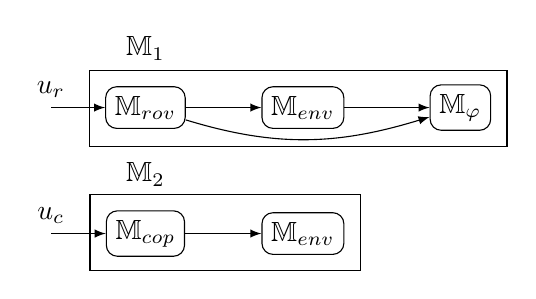
\begin{tikzpicture}
    \node[draw, node distance=2cm, rounded corners] (rover) {$\MDP_{rov}$};
    \node[draw, node distance=2cm, rounded corners, right of=rover] (environment) {$\MDP_{env}$};
    \node[draw, node distance=2cm, rounded corners, right of=environment] (fsa) {$\MDP_\varphi$};

    \draw[-latex] (rover) --  (environment);
    \draw[-latex] (environment) --  (fsa);
    \draw[-latex] (rover) to[out=-17, in=197] (fsa);

    \draw ([xshift=-2mm, yshift=2mm]$(rover.north west)$) rectangle ([xshift=2mm, yshift=-2mm]$(fsa.south east)$) {};
    \node[above of=rover, node distance=0.75cm] {$\MDP_1$};

    \draw[latex-] (rover) -- ++(-1.2,0) node[coordinate] (west) {} node[above] {$u_r$};

    \node[below of=rover, draw, node distance=1.6cm, rounded corners] (copter) {$\MDP_{cop}$};
    \node[draw, node distance=2cm, rounded corners, right of=copter] (env2) {$\MDP_{env}$};

    \draw[-latex] (copter) --  (env2);

    \draw ([xshift=-2mm, yshift=2mm]$(copter.north west)$) rectangle ([xshift=2mm, yshift=-2mm]$(env2.south east)$) {};
    \node[above of=copter, node distance=0.75cm] {$\MDP_2$};

    \draw[latex-] (copter) -- ++(-1.2,0) node[coordinate] (west) {} node[above] {$u_c$};

  \end{tikzpicture}
\end{center}
  \caption{Illustration of aggregate systems $\MDP_1$ and $\MDP_2$ constructed as serial products, where $\MDP_{env}$ is itself a parallel product.}
  \label{fig:agg}
\end{figure}

We consider a two-asset mission consisting of a ground rover and a flying copter 

\subsection{Problem setup}

\paragraph{Abstract Robot Models}

We denote the location of robot and copter with $x_r \in \mathbb{R}^2$ and $x_c \in \mathbb{R}^3$. For a given domain $\X_r \subset \mathbb{R}^2$ and $\X_c \subset \mathbb{R}^3$ we introduce abstract states $\xi_r \in [\X_r]_{N_{rx}, N_{ry}}$ and $\xi_d \in [\X_c]_{N_{cx}, N_{cy}, N_{cz}}$, where e.g. $N_{rx}$ is the number of discrete states along the $x$ axis. 

We assume that both robots freely can move east, north, west, or south between the discrete states while remaining in the workspace, and that the copter can additionally adjust its elevation by moving up and down. With these assumptions we can model the rover with an MDP $\MDP_{rov}$ with $N_{rx} N_{ry}$ states and $4$ inputs, and the copter as an MDP $\MDP_{copt}$ with $N_{cx} N_{cy} N_{cz}$ states and $6$ inputs. In the following we fix $N_{rx} = N_{ry} = N_{cx} = N_{cy} = 10$ and $N_{cz} = 2$, i.e. both robots move on a 10x10 grid in 2D space, and the copter can fly at two different altitudes (in the following referred to as \emph{high} and \emph{low}).

\paragraph{Low-level Robot Controllers}

How quadrotors are controlled to move between discrete states. \red{Can we provide some guarantees under reasonable assumptions?}
\sofie{What are the options? Can you compute a barrier function ? Can you do something like lyapunov stability? Input output stability.. }
\paragraph{Environment Belief Model}

\begin{figure}
  \begin{center}
  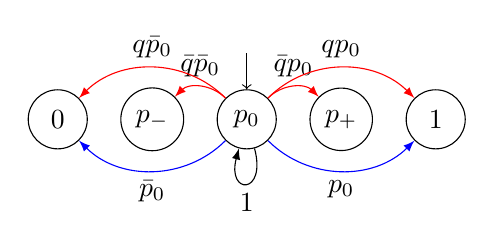
\begin{tikzpicture}
    \node[draw, minimum width=0.75cm, node distance=1.2cm, circle, initial above,initial text={} ] (bi) {$p_0$};
    \node[draw, minimum width=0.75cm, node distance=1.2cm, circle, left of=bi] (bm) {$p_-$};
    \node[draw, minimum width=0.75cm, node distance=1.2cm, circle, right of=bi] (bp) {$p_+$};
    \node[draw, minimum width=0.75cm, node distance=1.2cm, circle, right of=bp] (b1) {$1$};
    \node[draw, minimum width=0.75cm, node distance=1.2cm, circle, left of=bm] (b0) {$0$};

    \draw[-latex, red] (bi) to[out=45, in=135] node[black, above] {$\bar q p_0$} (bp);
    \draw[-latex, red] (bi) to[out=135, in=45] node[black, above] {$\bar q \bar p_0$} (bm);
    \draw[-latex, red] (bi) to[out=45, in=135] node[black, above] {$q p_0$} (b1);
    \draw[-latex, red] (bi) to[out=135, in=45] node[black, above] {$q \bar p_0$} (b0);
    \draw[-latex, blue] (bi) to[out=-45, in=-135]  node[black, below] {$p_0$} (b1);
    \draw[-latex, blue] (bi) to[out=-135, in=-45]  node[black, below] {$\bar p_0$} (b0);
    \draw[-latex, black] (bi) to[loop below] node[below, black] {1} (bi);
  \end{tikzpicture}
  \end{center}
  \caption{Illustration of environment belief model for a single region, only transitions from initial state $p_0$ are shown. Bars denote the complementary probability, i.e. $\bar p = 1-p$. When a high-quality measurement is received (blue edges), the belief transitions to $1$ with probability $p_0$ and to $0$ with probability $1-p_0$, whereas a low-quality measurement yields certainty with probability $q$ but with probability $1-q$ results in an intermediate belief $p_-$ or $p_+$. When no measurement is taken (black) the state does not change. The full transition matrices are given in}
  \label{fig:envmdp}
\end{figure}

We assume that regions of interest have been extracted from low-resolution satellite imagery, along with prior probability estimates for the likelihood that the regions exhibit certain traits. Here we restrict attention to \emph{risk regions} that may contain obstacles the rover can not traverse, and \emph{target regions} that are likely places where scientific samples can be extracted. We associate to each region $R_i$ a belief MDP $\MDP_{R_i}$ with five states $\zeta_i \in \{ 0, p^i_-, p^i_0, p^i_+, 1\}$ and three inputs $v_i \in \{ N, W, S \}$ for (N)o measurement, (W)eak measurement, and (S)trong measurement. The transition matrices are $T_N = I_5$, 
\begin{equation}
  T_{S} = \left[\begin{smallmatrix}
    1        &  0  &  0  &  0  &  0   \\
    \bar p_- &  0  &  0  &  0  &  p_- \\
    \bar p_0 &  0  &  0  &  0  &  p_0 \\
    \bar p_+ &  0  &  0  &  0  &  p_+ \\
    0        &  0  &  0  &  0  &  1
  \end{smallmatrix}\right],
  T_{W} = \left[\begin{smallmatrix}
    1        &  0                &  0  &  0           &  0   \\
    q\bar p_-&  \bar q \bar p_-  &  0  &  \bar q p_-  &  q p_- \\
    q\bar p_0&  \bar q \bar p_0  &  0  &  \bar q p_0  &  q p_0 \\
    q\bar p_+&  \bar q \bar p_+  &  0  &  \bar q p_+  &  q p_+ \\
    0        &  0  &  0  &  0  &  1
  \end{smallmatrix}\right].
\end{equation}
Here $q$ is a parameter denoting the quality of the weak measurement: if $q=0$ weak measurements are incapable of determining the true nature of the region, only intermediate beliefs $p_-$ and $p_+$ can be reached. For $q \in (0,1]$ there is a probability of a transition to a belief state 0 or 1. The outgoing transitions from $p_0$ are illustrated in Figure \ref{fig:envmdp}.

Given belief MDPs $\MDP_{R_i}$ for every region of interest, we construct the environment model $M_{env}$ as the parallel product
\begin{equation}
  \MDP_{env} = \MDP_{R_1} \otimes_{par} \MDP_{R_1}  \otimes_{par} \ldots \otimes_{par} \MDP_{R_n}. 
\end{equation}

\paragraph{Specification}

The objective of the mission is to satisfy a scLTL specification $\varphi$ over propositions over states in $\MDP_{rov}$ and $\MDP_{env}$. Examples of such propositions include
\begin{itemize}
  \item Don't enter a risk region $R_1$ that may contain an obstacle: $\xi_r \not  \in R_1 \lor \xi_1 = 0$.
  \item Collect a sample at region $R_2$: $\xi_r \in R_2 \land \xi_2 = 1$.
\end{itemize}

We posit that the rover has a time window of length $T_r$ to fulfill its mission, and that the copter has battery sufficient to operate for a time $T_c$. In addition, the copter must land in a pre-designated landing area $X_l$ at the end of the execution. Given these constraints, the challenge is to find strategies for both the copter and rover that maximize the probability that the science specification is fulfilled.


\subsection{Turn-based solution}

We decouple the problem by letting the copter execute first, followed by the rover. The goal of the copter is then one of exploring the uncertain environment in a way that maximizes the probability of success in the rover's execution. To solve this problem via sequential value iteration we convert the scLTL specification into a DFSA $\MDP_{\varphi}$ and consider the following two product systems:
\begin{equation}
\begin{aligned}
  \MDP_{1} &= \left( \MDP_{rov} \otimes_{ser} \MDP_{env} \right) \otimes_{ser} \MDP_{\varphi}, \\
  \MDP_{2} &= \MDP_{cop} \otimes_{ser} \MDP_{env}.
\end{aligned}
\end{equation}
The serial connections are defined via connections that map the state of one system to the output of the next. These connections are defined as follows:
\begin{itemize}
  \item If the rover is adjacent to a region $R_i$ it triggers a (S)trong measurement of that region,
  \item If the copter is at low altitude and in region $R_i$, it triggers a (S)trong measurement of that region,
  \item If the copter is at high altitude and within distance $2$ of region $R_i$, it triggers a (W)eak measurement of that region,
  \item The connection between the $\MDP_{rov} \otimes_{ser} \MDP_{env}$ product and $\MDP_{\varphi}$ is given by the truth value of atomic propositions for the state $(\xi_r, \xi_e)$.
\end{itemize}
Figure \ref{fig:agg} illustrates the two systems. We assume that the initial position $\xi_r^0$ of the rover is known, and let $\xi_\varphi^0$ be the initial state of the specification automaton. We propose the following two-step solution:
\begin{enumerate}
  \item For $\xi_1 = (\xi_r, \xi_e, \xi_\varphi)$ let $g(\xi_1', v') = \max( \ind_{X_f}(\xi_\varphi'), v' )$ and compute the value functions $V^1_t(\xi_1)$ for $t = T_r, T_r-1 \ldots, 0$ via the Bellman iterations
  \begin{equation}
  \label{eq:valit1}
  \begin{aligned}
      V^1_{T_r}(\xi_1) & = g(\xi_1, 0), \\
      V^1_{t-1} (\xi_1) & = \max_{u_r} \sum_{\xi_1'} T(\xi_1' \mid \xi_1, u_r) g(\xi_1', V_t(\xi_1')).
  \end{aligned}
  \end{equation} 
  \item For $\xi_2 = (\xi_c, \xi_e)$, compute the value functions $V^2_t(\xi_2)$ for $t = T_c, T_c-1, \ldots, 0$ via the Bellman iterations
  \begin{equation}
  \label{eq:valit2}
  \begin{aligned}
    V_{T_c}^2(\xi_2) & = \ind_{X_l} (\xi_c) \times V^1_0(\xi_r^0, \xi_e, \xi_\varphi^0), \\
    V_{t-1}^2(\xi_2) & = \max_{u_c} \sum_{\xi_2'} T(\xi_2' \mid \xi_2, u_c) V^2_t(\xi_2').
  \end{aligned}
  \end{equation}
\end{enumerate}
The interpretation of these value functions are as follows: $V_t^1(\xi_r, \xi_e, \xi_\varphi)$ is the probability that the rover will satisfy its mission if at time $t$ the state of the rover-environment belief-specification automaton system is $(\xi_r, \xi_e, \xi_\varphi)$. The copter is tasked with maximizing this probability at the initial states $\xi_r^0, \xi_\varphi^0$ that the rover \emph{can not affect}, by updating the belief $\xi_e$ that it \emph{can affect} via environment exploration in the way most beneficial for the rover. In addition, the requirement that the rover must be in the landing zone $X_l$ at time $T_c$ has been incorporated in the value function. Thus, $V_t^2(x_c, x_e)$ represents the probability that the rover will have a successful execution, and that the copter can land in $X_l$, if the copter-environment state at time $t$ is $(x_c, x_e)$. In addition to the value functions, time-dependent policies that maximize the value functions can be extracted as the maximizing argument.

Both iterations \eqref{eq:valit1} and \eqref{eq:valit2} fall within the framework of sequential value iteration for parallel and serial products in Section \ref{sec:sequential_val_iter}. As a consequence there is no need to construct the aggregate transition matrices for $\MDP_1$ and $\MDP_2$.


\subsection{Illustrations}

We demonstrate the features of the proposed solution in a few example scenarios.

\paragraph{Scenario 1} Collect one sample of type $A$ and one sample of type $B$ while avoiding obstacles:
\begin{equation*}
  \left( \lnot \texttt{obstacle} \; \mathcal U \; \texttt{sampleA} \right) \land \left( \lnot \texttt{obstacle} \; \mathcal U \; \texttt{sampleB} \right)
\end{equation*}
The maximum execution lengths are 15 for the rover and 20 for the copter, and the copter must return to its initial state at the end of its execution. Figure \ref{fig:workspace1} illustrates the workspace and Figure \ref{fig:values1} the resulting value functions. In this environment, the success probability for the rover is 12.4\% if copter-aided exploration is not available, as reflected by the purple color in the lower left corner of Figure \ref{fig:values1}. However, copter exploration lifts the success probability to 29.4\%. Note that this is the probability of success without assuming any additional information about the environment---the joint probability that a sample of type $A$ exists and that sample $B$ can be accessed is $0.64 \times 0.75 = 0.48$, which is thus an upper bound on the success probability of this mission. The increased success probability is solely due to the fact that the copter can explore, thus alleviating the rover from having to guess the true nature of the environment.

\begin{figure}
  \begin{center}
    \includegraphics[width=0.6\columnwidth]{2figs/exp1-map.pdf}
  \end{center}
  \caption{Workspace where regions of interest $R_i$, $A_i$, and $B_i$ are marked for risk regions, sample A targets, and sample B targets, along with associated prior probabilities. The initial states $\xi_r^0$ and $\xi_c^0$ are marked, as well as the green region where the copter can safely land. Regions with $p=1$ are known and thus not modeled with belief state.}
  \label{fig:workspace1}
\end{figure}

\begin{figure}
  \begin{center}
    \footnotesize
    \begin{tikzpicture}
      \node[inner sep=0] (p1) {\includegraphics[height=0.24\columnwidth]{2figs/value-rov.pdf}};
      \node[inner sep=0, anchor=west] at ([xshift=2mm]$(p1.east)$) (p2) {\includegraphics[height=0.24\columnwidth]{2figs/value-cop.pdf}};
      \node[inner sep=0, anchor=west] at ([xshift=2mm]$(p2.east)$) (n1) {
\includegraphics[height=0.24\columnwidth]{2figs/cbar.pdf}};
      \node at ([yshift=2mm]$(p1.north)$) {$V_0^1(\xi_r, \xi_e^0, \xi_\varphi^0)$};
      \node at ([yshift=2mm]$(p2.north)$) {$V_0^2(\xi_c, \xi_e^0)$};
      \node at ([xshift=6mm]$(n1.north east)$) {$p = 0.48$};
      \node at ([xshift=6mm]$(n1.south east)$) {$p = 0$};
    \end{tikzpicture}
  \end{center}
  \caption{Illustration of value functions. As can be seen, the advantage of the copter is equivalent to having the rover's initial state be near a target region.}
  \label{fig:values1}
\end{figure}

\section{Hardware Experiments}

\begin{itemize}
    \item Copter in CAST
\end{itemize}

\printbibliography

\end{document}

